\documentclass[../main.tex]{subfiles}

\begin{document}
\section{The theory of homology}
% TODO: Write paragraph contextualising the theory of hoomlogy

\subsection{The algebraic side: chain complexes and homology groups}
The basic object in the theory of homology is a \emph{chain complex}, which consists of a
family of abelian groups \( \set{C_n}_{n \in \N} \) together with a family of morphisms \(
\partial_n \colon C_n \to C_{n-1} \) such that \( \partial_n \circ \partial_{n+1} \). We
can then define the space of \emph{\( n \)-cycles} as \( \ker{\partial_n} \) and the space
of \emph{\( n \)-boundaries} as \( \im{\partial_{n+1}} \). The \emph{\( n \)-th homology group}
of the complex is then
\begin{equation*}
	H_n \defeq \ker{\partial_n} / \im{\partial_{n+1}}. 
\end{equation*}

\subsection{Simplices and simplicial complexes}
For the purposes of data analysis, the simpler theory of simplicial homology. As we will
see, it can be framed in purely combinatorial terms which is very useful when it comes to
computation. 

The basic geometric building block is the simplex. This is the generalisation of a
triangle in two dimensions and a tetrahedron in three dimensions. 

\begin{definition}[Simplex]\label{def:simplex}
	A simplex of dimension \( n \), or simply an \( n \)-simplex, generated by \( n+1 \)
	points of \( \R^d \) which do not lie in an affine subspace of dimension \( n
	\)\footnote{which means the ambient dimension \( d \) must be at least \( n \)}, is
	their convex hull, i.e. the smallest convex set which contains them.
\end{definition}

The \( n \)-simplex generated by the points the standard basis of \( \R^{n+1} \), \( e_0,
\dots, e_n \)\footnote{Because an \( n \)-simplex is generated by \( n+1 \)-points, it
will be convenient to number things starting at 0, as opposed to 1 as is more common in
the rest of mathematics}, is called the \emph{standard \( n \)-simplex} and
written \( \Delta^n \). It is easy to show that
\begin{equation*}
	\Delta^n = \set{(t_0, \dots, t_n) \in \R^{n+1} \mid \sum_{k = 0}^{n} t_k = 1, \forall k
	\leq n \colon t_k \geq 0}. 
\end{equation*}
The standard simplices provide a model for any other simplex. Indeed, if \( \phi \colon
\R^{n+1} \to \R^d \) is the linear map defined by \( \phi(e_k) = p_k \) for \( 0 \leq k
\leq n \) then \( \phi(\Delta^n) \) is precisely the simplex generated by \( p_0, \dots,
p_n \). \( (t_0, \dots, t_n) \) are called the \emph{barycentric coordinates} of the point
\( \phi(t_0, \dots, t_n) \). 

\paragraph{Orientation.}
For the purposes of homology, it is also important to keep track of the \emph{orientation} of a
simplex. We will use the idea of general simplices being the image of standard simplices
to model this situation
\begin{definition}[Ordered simplex]
	An \emph{ordered \( n \)-simplex} generated by \( p_0, \dots, p_n \in \R^d \) is a map
	\( \sigma \colon \Delta^n \to \R^d \) such that \( \sigma \) is the restriction to \(
	\Delta^n \) of the linear map \( \phi \colon \R^{n+1} \to \R^d \) given by \( \phi(e_k)
	= p_k \), provided \( p_0, \dots, p_k \) do indeed generate a simplex. 
\end{definition}
Observe that giving an ordering to the vertices of a simplex completely determines an
ordered simplex, thus we introduce the notation \( [p_0, \dots, p_n] \) for an ordered
simplex as defined above. 

Consider now the natural action of the symmetric group, \( \S_n \), on \( \R^n \) by permuting the elements of
the standard basis. Thus, a reordering of an ordered \( n \)-simplex \( \sigma \) is of
the form \( \tau \circ \sigma \) for some \( \tau \in \S_{n+1} \). We will then say that
two simplices \( \sigma_1 \) and \( \sigma_2 \) have the same \emph{orientation} if there
exists an even permutation \( \tau \in \S_{n+1} \) such that \( \sigma_1 = \tau \circ
\sigma_2 \). It then follows, because the even permutations are an index 2 subgroup of \(
\S_n\), that any \( n \)-simplex only has two possible orientations, as happens with
manifolds, for instance. See \cref{fig:orientation} for an example. 

\begin{figure}[htb]
	\centering
	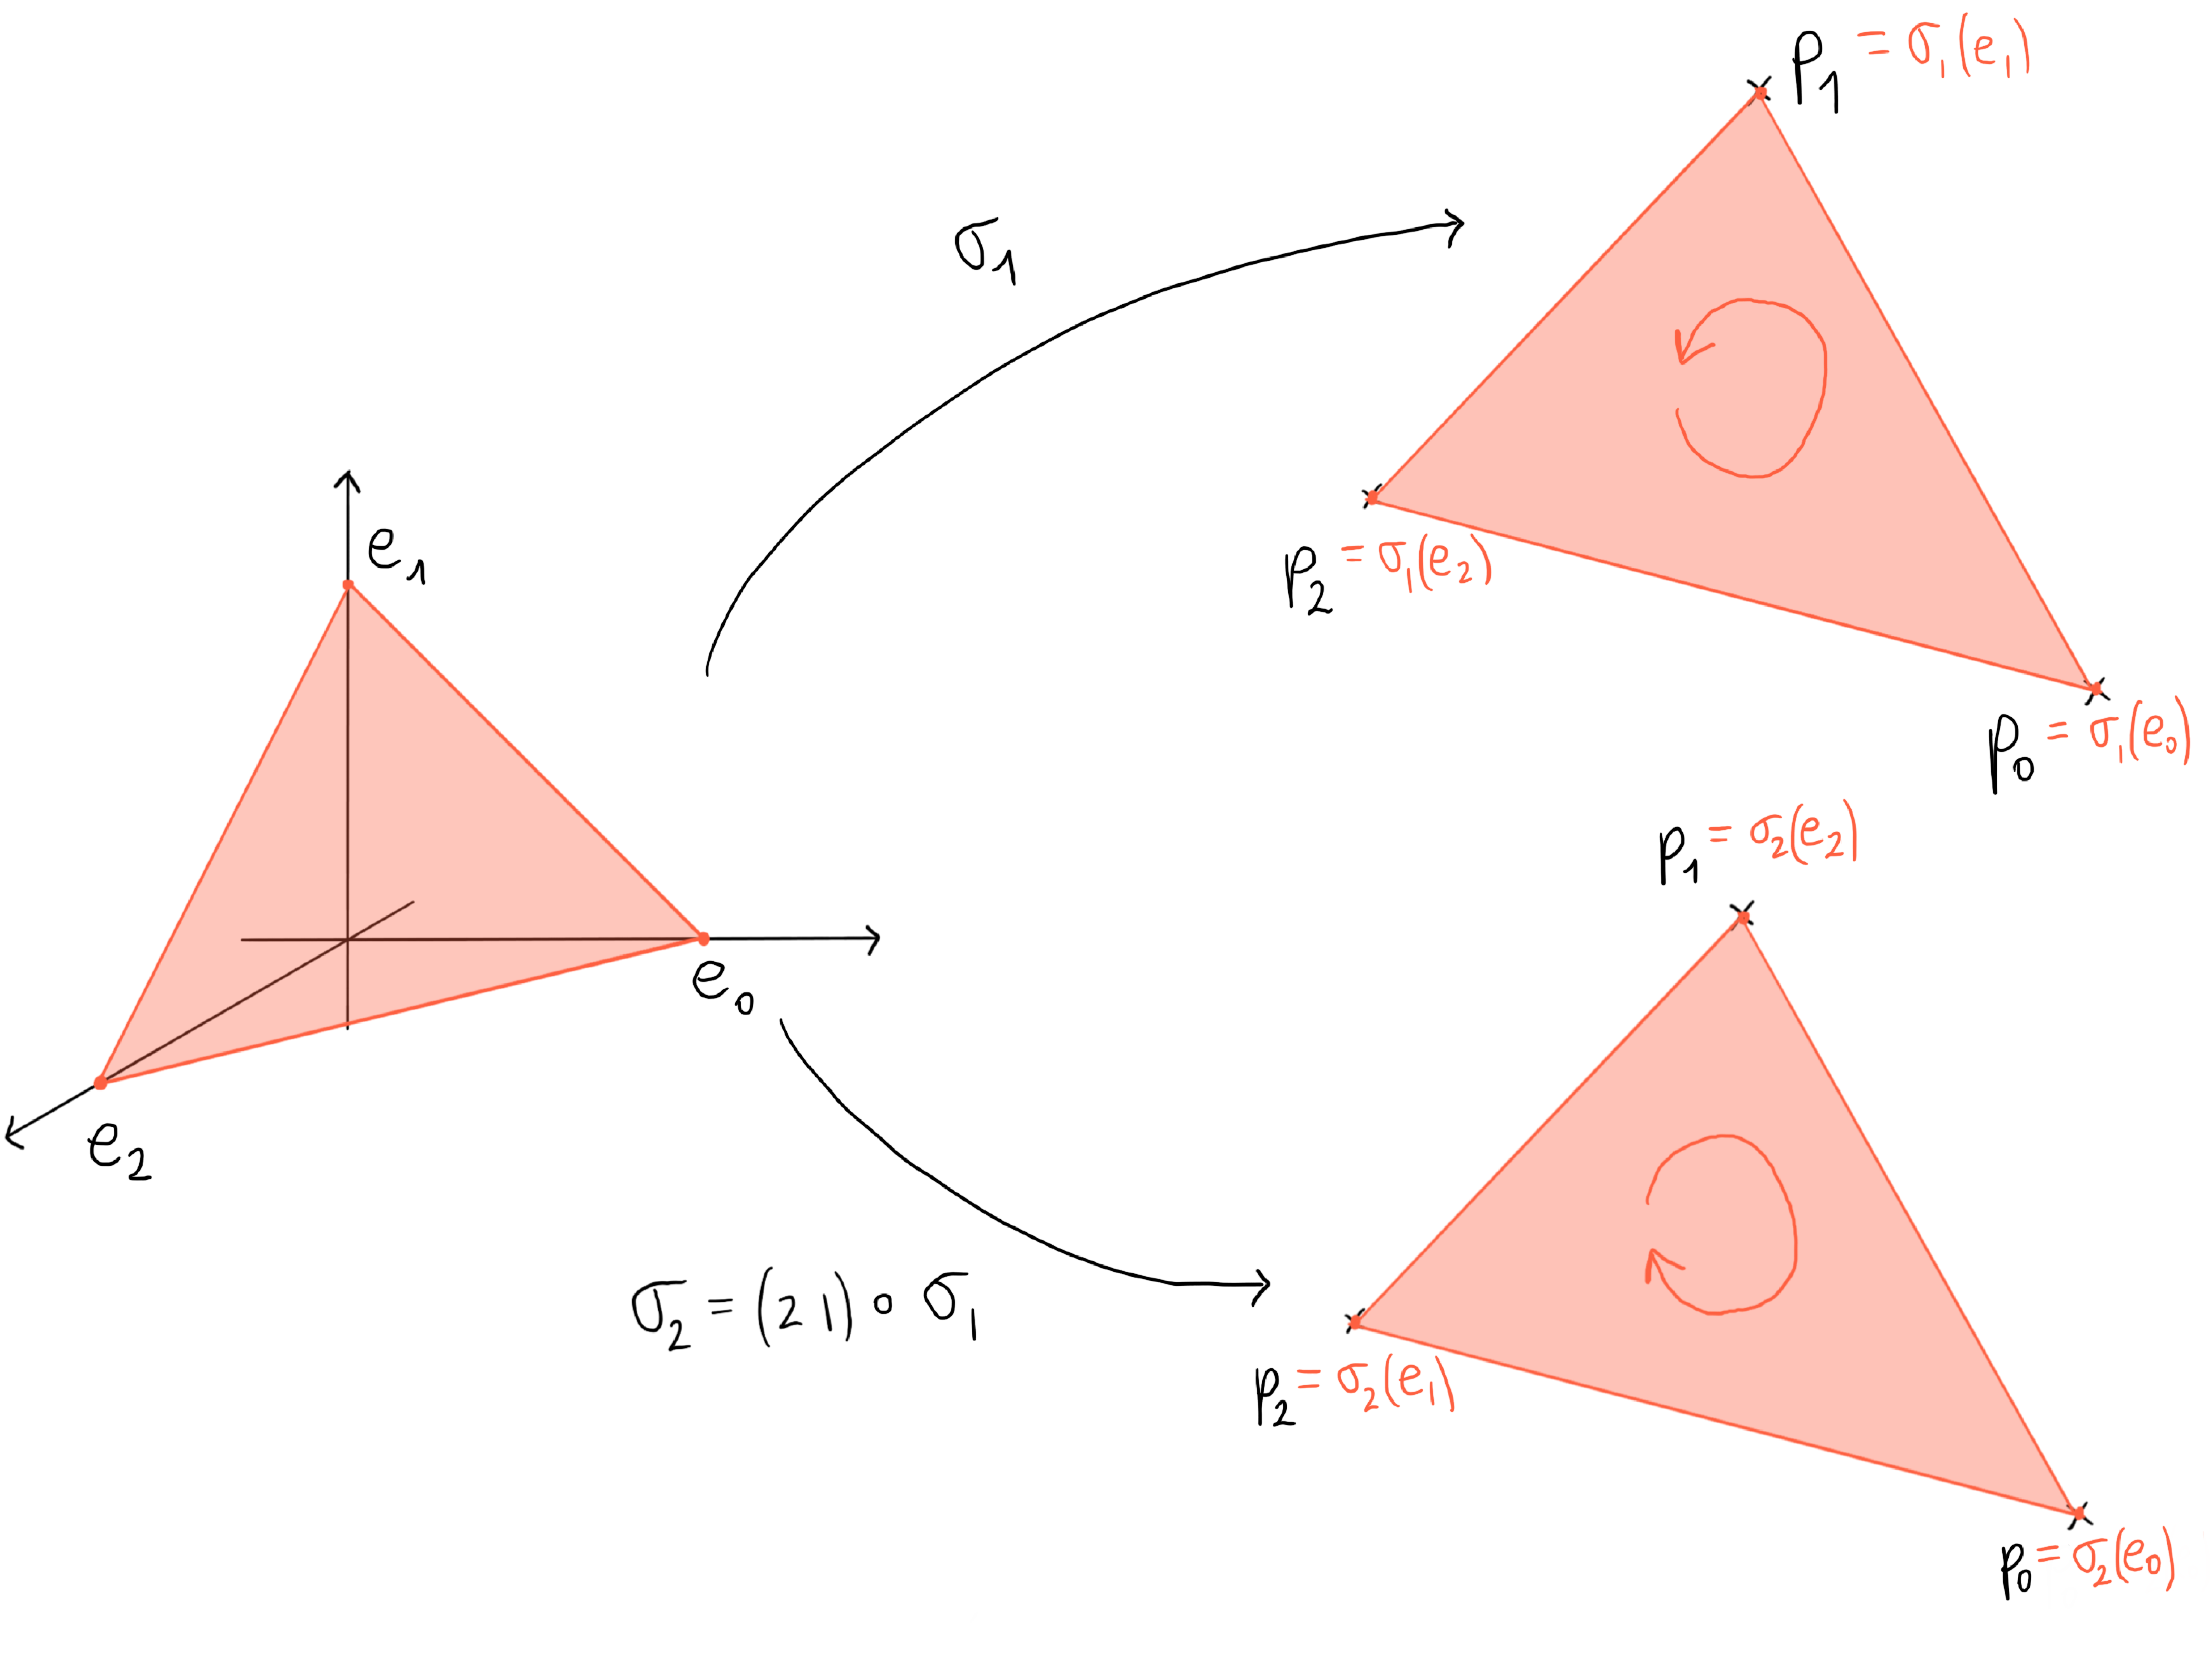
\includegraphics[width = 10cm]{figs/orientation}
	\caption{Two different orderings of a 2-simplex with the same vertices that determine
	different orientations.}
	\label{fig:orientation}
\end{figure}

The faces of an \( n \)-simplex, \( \sigma \), are the \( n+1 \) possible \( n-1
\)-simplices generated by all but one of the vertices of \( \sigma \). 

% TODO: Finish

Given a simplex \( \sigma = [p_0, \dots, p_n] \), the \( n+1 \) possible simplices we get by
removing one of the generators ---i.e. \( [p_1, \dots, p_n] \) and so on--- are called the
\emph{faces} of \( \sigma \). In barycentric coordinates, they correspond to setting one of the
coordinates equal to 1. 

\begin{definition}[Simplicial complex]\label{def:simplicial complex}
	A \emph{simplicial complex} \( K \) is a collection of simplices of \( \R^d \) such that 
	\begin{enumerate}[(i)]
		\item if \( \sigma \in K \) and \( \tau \in K \) is a face of \( \sigma \) then \(
			\tau \in K \),
		\item for any \( \sigma, \tau \in K \) then \( \sigma \cap \tau \in K \). 
	\end{enumerate}
\end{definition}
The intuition is that the simplices that make up a simplicial complex are glued together
only along their faces. 

The simplices of \( K \) are often called its \emph{cells}, and we will write \( K^n \)
for collection of \( n \)-cells of \( K \). 

A simplicial complex \( K \) determines a topological space, called its \emph{underlying
space}, which is the subset of \( \R^d \) determined by the union of all of the cells of
\( K \) equipped with the subspace topology, which we will write as \( \abs{K} \). The
theory of homology built using this class of spaces is known as \emph{simplicial
homology}. It should be noted, however, that homology can be implemented on much more
general spaces by considering continous maps from the standard simplices into the space,
which leads to the theory of singular homology. 

\subsection{Abstract simplicial complex}
Notice that a simplex is always determined by its vertices, and vice versa, except for, of
course, whenever the vertices do not generate a simplex, in the sense of
\cref{def:simplex}. This requirement comes from thinking of simplices and simplicial
complexes as geometric objects. But if we don't think of them in this way, and simply
allow for any \( n+1 \) vertices to determine an \( n \)-simplex they become strictly
combinatorial objects. In this case, we also have to lift the second condition in the
definition of a simplicial complex, which was related to how the simplices are assembled
together as geometrical objects and therefore is senseless in this new context. This more
general complexes are called \emph{abstract simplicial complexes} and are purely
combinatorial objects. From this viewpoint, the faces of a simplex are simply subsets of
its vertices, thus, \cref{def:simplicial complex} now becomes
\begin{definition}[Abstract simplicial complex]
	An \emph{abstract simplicial complex} \( K \) is any set closed under the relation of
	inclusion, i.e., if \( \sigma \in K \) then if \( \tau \subseteq K \), it must be the
	case that \( \tau \in K \).  
\end{definition}
For our purposes, we will assume that all of the simplices that make up a complex are
finite, that there is a maximum possible dimension  and that complexes are at most
countably infinite, thus avoiding problems related to size. 

Notice that to specify a complex it suffices to exhibit its \emph{maximal simplices},
those simplices which are not the face of any other simplex, or equivalently those which
are maximal with respect to inclusion\footnote{This is guaranteed by requiring that the
dimensions of all simplices that make up the complex be bounded.}.

For the purposes of homology, we will need to define some notion of orientation for a
simplex. For the case of 1-simplices this is evident, simply pick one of the two orderings
of its two vertices. For 2-simplices, if we think back to the geometrical picture, we
could think of the clockwise and counterclockwise orientations. Then, any two possible
orderings of the vertices give the same orientation if they are related by an even
permutation, thus there are two possible orientations. This is easily generalisable to
arbitrary dimension, and so we will say that two orderings of the vertices of a simplex
have the same orientation if they differ by an even permutation, which implies there are
only two possible orientations.

\subsection{Special complexes}
In the context of topological data analysis, one often wants to give some sort of
geometric structure to a set of points, and a common way of doing this is by constructing
a simplicial complex out of them. There are various ways of achieving this, which we now
describe. For the remainder of this section, \( X \) will denote a finite subset of \(
\R^d \), which models the raw point cloud we begin with. 

\paragraph{Čech complex.} The \( \epsilon \)-Čech complex of \( X \), \( C_\epsilon(X) \),
is determined by the following prescription: \( \sigma \subseteq X \) is in \(
C_\epsilon(X) \) if and only if \begin{equation*} \bigcap_{p \in \sigma} B_\epsilon(p)
	\neq \emptyset \end{equation*} where \( B_\epsilon(p) \) is the ball of radius \(
	\epsilon \) centered at \( p \). 

\paragraph{Vietoris-Rips complex.} The prescription for the \( \epsilon \)-Vietoris-Rips
complex, \( V_\epsilon(X) \), is as follows: \( \sigma \subseteq X \) defines a simplex in
\( V_\epsilon(X) \) if and only if for every \( p, q \in \sigma \) 
\begin{equation*}
	B_\epsilon(p) \cap B_\epsilon(p) \neq \emptyset.
\end{equation*}
In other words, a set of points generate a simplex whenever each of them is at distance at
most \( 2\epsilon \)\footnote{Some texts use a slightly different convention such that the
vertices of a clique in	\( V_\epsilon(X) \) are at distance at most \( \epsilon \) (rather
than \( 2\epsilon \)) from each other} from the rest. 

Notice that the \( \epsilon \)-Čech complex is always a subcomplex of the \( \epsilon
\)-Vietoris-Rips complex. 

\paragraph{Clique complex.} If the points of our cloud are the vertices of some graph, \(
G \), we can use this information to build the so-called clique complex, \( G(X)
\), by declaring that \( \sigma \subseteq X \) is a simplex of \( G(X) \) if and
only if it is a clique, i.e. a fully-connected subgraph of \( G \). The Vietoris-Rips
complex is a special case of this, since it is the clique complex of the graph obtained by
declaring to points of \( X \) adjacent when they are at distance at most \( 2\epsilon \).
This is the main c

\subsection{Simplicial chain complexes and homology groups}
Once we have the geometric ideas in place, we can start constructing the algebraic
objects. As we discussed, we want to define a structure that captures (at least some of
the) information encoded in the fundamental groups, but which is also algebraically
simpler. Given a simplicial complex \( K \), we can consider the free abelian group of
(oriented) \( n \)-cells. In the case of \( n = 1 \) this is, in some sense which can be
made precise, related to the abelianisation of the first fundamental group. 

We want the orientation to play nicely with the group structure, so the group will not be
totally free as we will require that for any oriented simplex \( \sigma \), \( -\sigma \)
is the simplex with the same vertices but opposite orientation. This group is called the
\( n \)-th simplicial chain group of the complex, \( C_n(K) \). 

The next step towards constructing the homology groups is defining the boundary morphisms.
\begin{definition}[Boundary morphisms]
	We define, for \( n \geq 1 \), the morphisms
	\begin{equation*}
		\partial_n \colon C_n(K) \longto C_{n-1}(K)
	\end{equation*}
	by giving their action on an arbitrary generator as
	\begin{equation*}
		\partial_n [p_0, \dots, p_n] \defeq \sum_{k = 0}^{n} (-1)^k [p_0, \dots, \hat p_k,
		\dots, p_n]. 
	\end{equation*}
\end{definition}
We need to show that all of this is indeed a chain complex, which is a consequence of the
following result.
\begin{lemma}
		For any \( n > 1 \), \( \partial_{n-1} \circ \partial_n = 0 \). 
\end{lemma}
\begin{proof}
	It suffices to show this on any generator, which is a simple calculation:
	\begin{align*}
		(\partial_{n-1} \circ \partial_n)[p_0, \dots, p_n] = {} & \partial_{n-1}\left(\sum_{k
		=		0}^{n}(-1)^k[p_0, \dots, \hat p_k, \dots, p_n]\right) \\
				= {} & \sum_{k = 0}^{n}(-1)^k	\partial_{n-1}[p_0, \dots, \hat	p_k, \dots, p_n] \\
				= {} & \sum_{k = 0}^{n}(-1)^k	\left(\sum_{l = 0}^{k - 1} (-1)^l [p_0, \dots, \hat	p_l, \dots, \hat p_k, \dots, p_n] \right. \\
						 & {} + \left. \sum_{l = k+1}^{n}(-1)^{l-1} [p_0, \dots, \hat p_k, \dots, \hat
						 p_l \dots, p_n]\right) \\
				= {} & \sum_{\mathclap{\substack{k = 0 \\ l < k}}}^n (-1)^k(-1)^l [p_0,	\dots,
				\hat p_l, \dots, \hat p_k, \dots, p_n] \\
						 & {} - \sum_{\mathclap{\substack{k = 0 \\ l > k}}}^n (-1)^k(-1)^l [p_0,
						 \dots, \hat p_k, \dots, \hat p_l, \dots, p_n] \\
				= {} & 0
	\end{align*}
	because both summands in the last line are the same. 
\end{proof}
We will drop the subscripts from the boundary morphisms whenever they can be deduced from
the context. 

\begin{figure}[htb]
	\centering
	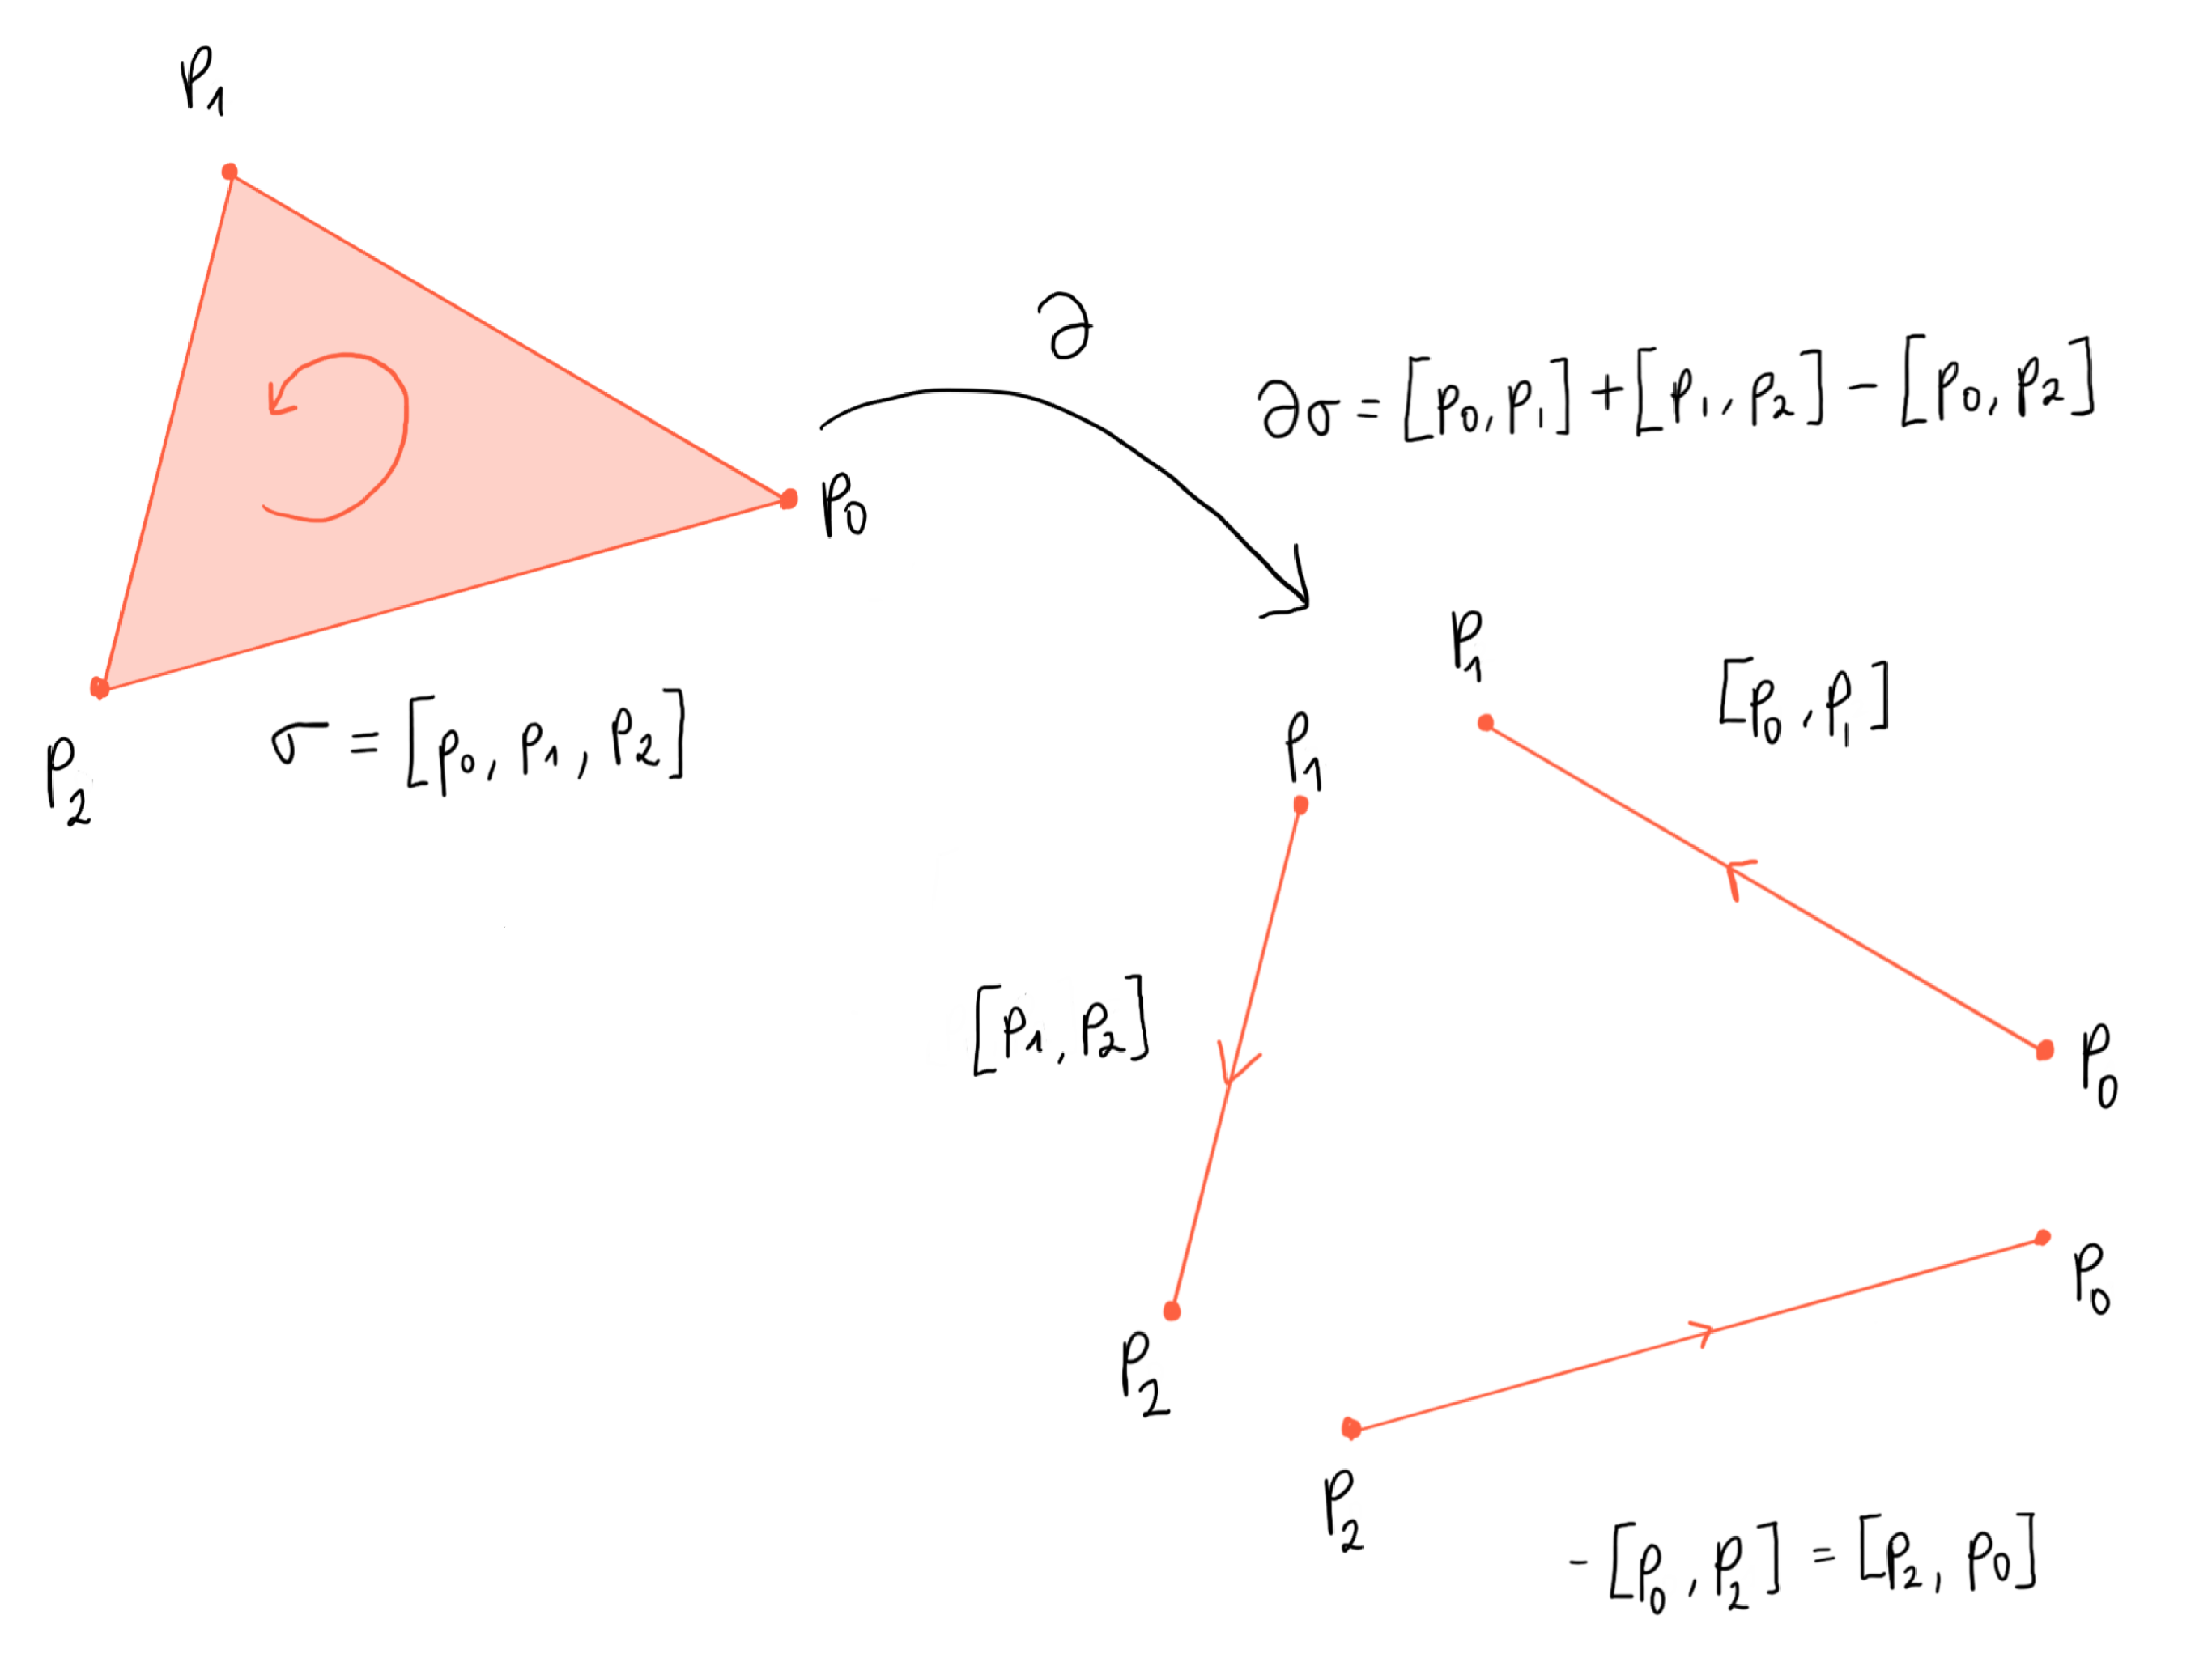
\includegraphics[width = 12cm]{figs/boundary}
	\label{fig:boundary}
\end{figure}

Thus, if \( d \) is the maximum dimension of the simplices of \( K \), we have the
simplicial chain complex
\begin{equation*}
	\begin{tikzcd}
		C_d(K) \arrow[r, "\partial_d"] & C_{d-1}(K) \arrow[r] & \cdots \arrow[r] & C_1(K)
		\arrow[r, "\partial_1"] & C_0(K) \arrow[r] & 0 
	\end{tikzcd}
\end{equation*}
thus we can immediately define the simplicial homology groups by
\begin{equation*}
	H_n(K) \defeq \ker \partial_n / \im \partial_{n+1}. 
\end{equation*}

A variant of this is, instead of defining the chain groups as free abelian groups,
defining the chain groups as vector spaces over a field \( F \) generated by the oriented
simplices ---with the condition that \( -\sigma \) is \( \sigma \) with the opposite
orientation---, which would be more sensibly called chain spaces. Thus the homology groups
would become homology spaces, which then allows for the definition of the \emph{Betti
numbers}:
\begin{equation*}
	\beta_n(X) = \dim H_n(X, F)
\end{equation*}

So what kind of innformation do we get from looking at the homology of a space?
The 0th Betti number is exactly the number of connected
components of the space. And the higher Betti numbers are, essentially, the number of
higher-dimensional holes in the space. The best way to understand this is by looking at the
homology of various common spaces. Of course, we have only developed the theory for
simplicial complexes, but there are ways homology can be defined for (somewhat
well-behaved) spaces. 

The homology of \( \R^n \) is 

\section{The idea of persistence}
So far we have seen various ways of extracting information related to the shape of our
data using homology. All of this ways, however, carry with them an ammount of arbitrary
choice. For example, both the Vietoris-Rips and Čech complexes depend on a scale parameter
\( \epsilon \), and the appropriate choice of \( \epsilon \) is generally not clear from
the data. The idea of persistent homology is to sidestep this problem altogether by
considering the homology of the data at every scale, to determine which are the features
really reflect geometric aspects and which are byproducts of background noise. The first
will be, roughly speaking, those which are present ar a large range of scales, i.e. those
which are \emph{persistent}. We now formalise these ideas.

\subsection{Filtrations}
\begin{definition}[Filtration]
	A \emph{filtration} is a family of simplicial complexes \( \set{K_i}_{i = 0}^n \)	such
	that \( K_i \) is a subcomplex of \( K_{i+1} \),
	\begin{equation*}
		K_0 \subseteq K_1 \subseteq \cdots \subseteq K_n
	\end{equation*}
	where we will mostly assume \( K_0 = \emptyset \). 
\end{definition}
The inclusions \( \iota_i^j \colon K_i \into K_j \), because of the functoriality of homology, give
rise to maps between the homology groups at different steps of the filtration,
\begin{equation*}
	H_p(\iota_i^j) \colon H_p(K_i) \longto H_p(K_j)
\end{equation*}
which we will write as \( f_i^j \) for short. We say a certain class is \emph{born at \( i
\)} if it is not in the image of any \( f_k^i \) for any \( k \leq i \). And we say it
\emph{dies at \( j \)} if it is in the kernel of \( f_i^j \) but not of \( f_i^k \) for \(
k < j \). The difference \( j - i \) is called its \emph{persistence} or \emph{lifetime}. 

This is a reflection at the level of homology of how the shape of the complex changes at
every step of the filtration. 







\end{document}
